\begin{solution}{normal}\textbf{(a)} The power received by plate is equal to the power received by lens  or $\pi\left(\frac{d}{2}\right)^2I$
\begin{center}
    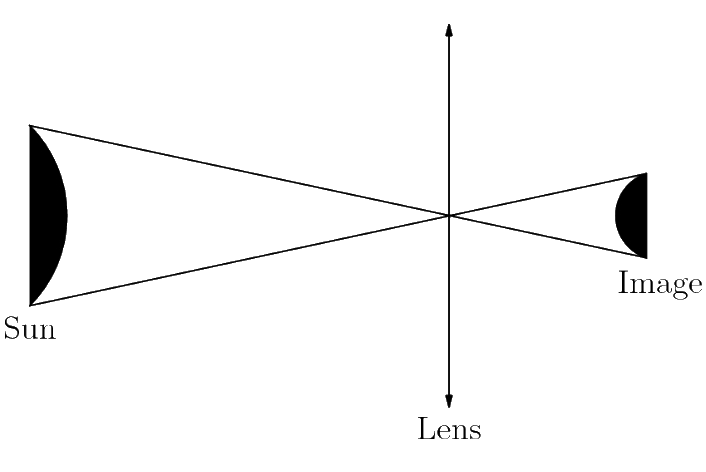
\includegraphics[width=12cm]{0A5C0D21-84E2-4E18-9164-078E0A965068.png}
\end{center}
With small angle approximations, the radius of the image is approximately $f\alpha/2$. Therefore, the power radiated by image $\pi\left(\frac{f\alpha}{2}\right)^2\sigma T^4$. In thermodynamic equilibrium the power received is equal to the power radiated. This then implies that 
\[ \frac{\pi d^2}{4} I = \frac{\pi f^2 \alpha^2}{4}\sigma T^4\implies T = \sqrt {\frac{d}{\alpha f}\sqrt {\frac{I}{\sigma}}}.\]
\vspace{3mm}

\noindent \textbf{(b)} At the sun’s surface the intensity of the sun is given by $$I_{\text{sun}} = \sigma T_{\text{sun}}^4\implies 4I_{\text{Sun}}\pi R_{\text{Sun}}^2 = 4 I \pi R_{\text{Orbit}}^2$$
where $R_{\text{Orbit}}$ is the orbital distance of Earth from Sun. This means that
$$I = \frac{\sigma T_{\text{Sun}}^4 R_{\text{Sun}}^2}{R_{\text{Orbit}}^2}$$
By Second Law of Thermodynamics temperature of plate can’t be more than temperature of Sun.
Therefore, $$T \leq T_{\text{Sun}}\implies \frac{d}{\alpha f}\sqrt {\frac{I}{\sigma}} \leq T_{\text{Sun}}^2\implies \frac{d}{\alpha f} \times \frac{T_{\text{Sun}}^2 R_{\text{Sun}}}{R_{\text{Orbit}}} \leq T_{\text{Sun}}^2\implies \frac {d}{\alpha f} \frac{\alpha}{2}\leq 1 \implies \boxed {d \leq 2f}.$$


\end{solution}